\mkImg{image copy 3} 
\^{} Flushing TLB \& pipeline flushing

\hSep

\textcolor{cornellred}{UNIX allows processes to create hierarchies.} 
\textcolor{ceruleanblue}{Windows has no notion of this.}

\textcolor{cornellred}{
\textit{\textbf{int fork(void)}} — Creates new child process, to be executed
concurrently, by making exact copy (same resources) of
parent process image. Returns child PID in \textbf{parent} process
and 0 in \textbf{child} process. No child created, and -1
returned to parent on error.}

\textcolor{cornellred}{
\textit{\textbf{int execve(char *path, char *argv[], char *envp[])}} — Changes process image and runs new
process. Lots of useful wrappers.}

\textcolor{cornellred}{
\textit{\textbf{int waitpid(int pid, int* status, int options)}} — Suspends execution of calling process
until process \textit{pid} terminates normally or signal received.
Can wait for more than one child.}

\mkImg{image copy 5}
\mkImg{image copy 7}

\textcolor{cornellred}{
\textit{\textbf{void exit(int status)}} — Terminates a process. Never returns in the
calling process.}

\textcolor{cornellred}{
\textit{\textbf{int kill(int pid, int sig)}} — sends signal sig to process pid.}

\hSep

\begin{wrapfigure}[9]{l}{67pt}
\vspace{-12pt}
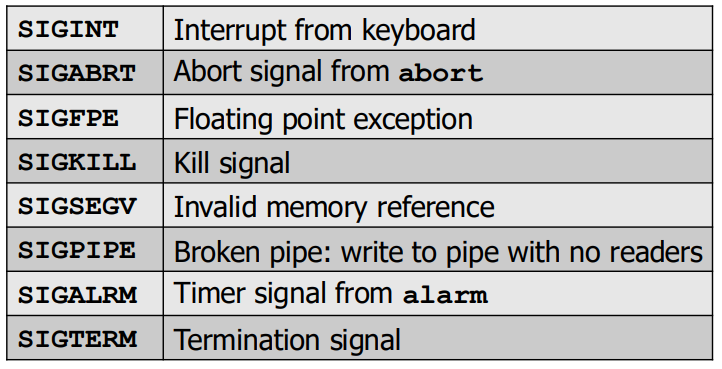
\includegraphics[width=70pt]{pastedimg1}
\end{wrapfigure}

\textcolor{cornellred}{\textbf{SIGNALS}} are an IPC mechanism — 
\textbf{delivery} similar
to delivery of hardware interrupts. Process can send signal to
another process, if it has permission. Generated when an
exception occurs, when kernel wants to notify process of
an event, when certain key combinations typed in terminal, 
or programmatically using \textcolor{cornellred}{\textit{int kill()}}.

\mkImg{image copy 4}

\mkImg{image copy 6}

\textcolor{cornellred}{\textit{\textbf{int pipe(int fd[2])}} — 
returns two file descriptors: 
read end \textit{fd[0]}, write end \textit{fd[1]}.}

\hSep

\mkImg{image copy 8}
\mkImg{image copy 9}

\textcolor{cornellred}{\textit{\textbf{void pthread\_exit(void \*value\_ptr)}} — 
Terminates the thread and makes \textit{value\_ptr} available to any successful join with terminating thread.
Called implicitly when the thread's start routine returns.}

\mkImg{image copy 10}
\mkImg{image copy 11}

\hSep